A dual-stacked host with native IPv6 connectivity establishing a TCP
connection to a dual-stacked web service prefers IPv6. This is because
\texttt{getaddrinfo(\ldots)} resolves a service name to a list of endpoints in
an order that prioritizes an IPv6-upgrade path \cite{rfc6724}.  The dictated
order can dramatically reduce the application's responsiveness in situations
where IPv6 connectivity is broken, because the attempt to connect over an IPv4
endpoint will take place only when the IPv6 connection attempt has timed out,
which can be in the order of seconds.

\begin{figure}[t]
\centering
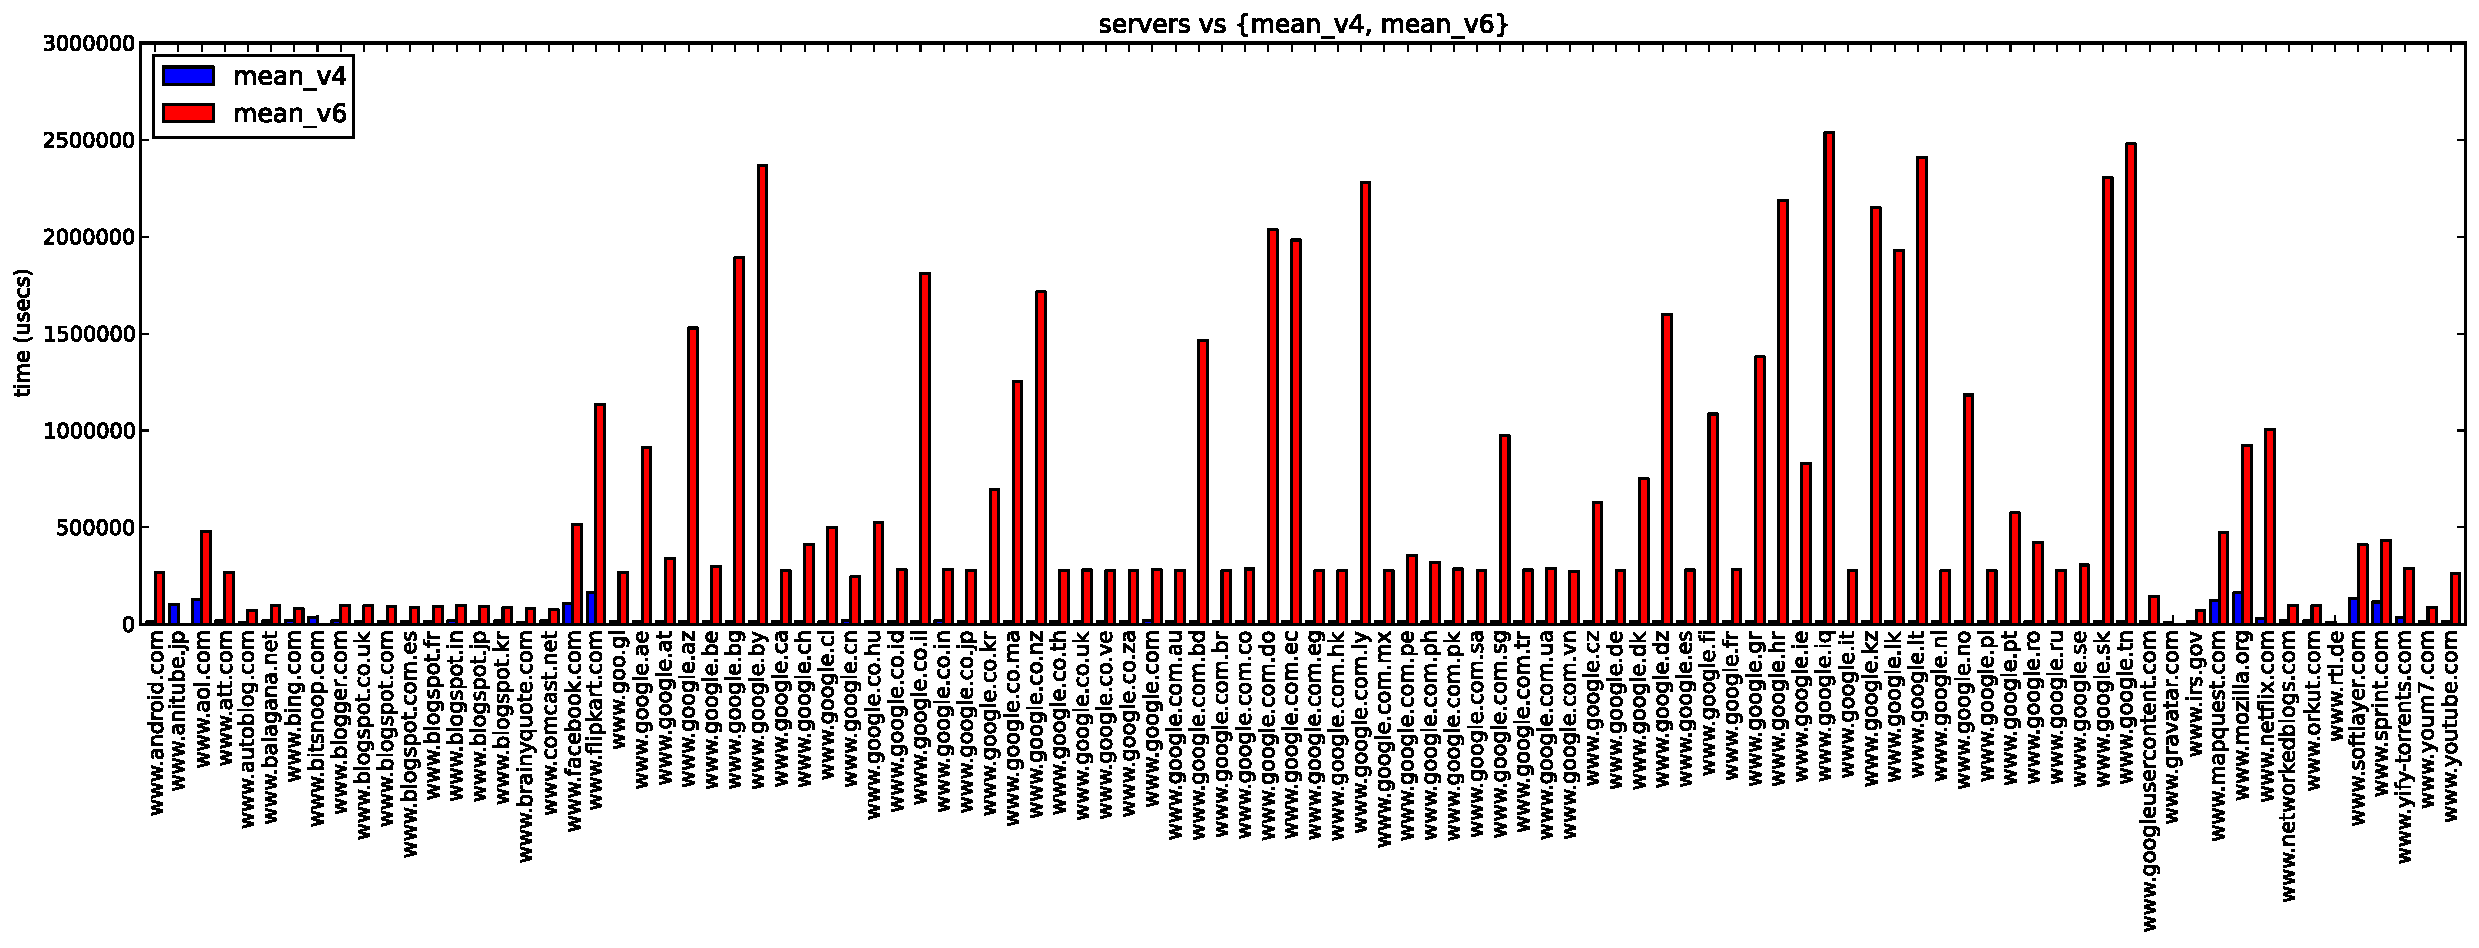
\includegraphics[width=1.0\textwidth]{figures/t28972-mean}
\caption{Mean time to establish TCP connections to a list of web services. The
measurement point is a virtual machine hosted at \texttt{greatnet.de}. It
has IPv4 connectivity via LamdaNet Communications [AS13237] and IPv6
connectivity via Teredo.}
\label{fig:t28972-mean}
\end{figure}

This noticeable degraded user experience can be subverted by implementing the
happy eyeballs algorithm \cite{rfc6555} in applications. The algorithm
recommends that a host, after resolving the DNS name of a dual-stacked
service, tries a TCP \texttt{connect(\ldots)} to the first endpoint (usually
IPv6). However, instead of waiting for a timeout, it only waits for 300ms,
after which it must initiate another TCP \texttt{connect(\ldots)} to an
endpoint with a different address family and start a competition to pick the
one that completes first.  In this pursuit, to determine whether applications
will use IPv4 or IPv6 on a dual stacked service, we developed \texttt{happy},
a simple TCP happy eyeballs probing tool. It uses non-blocking
\texttt{connect(\ldots)} calls to concurrently establish connections to all
endpoints of a service.  We have cross-compiled \texttt{happy} for the
OpenWrt\footnote{\url{http://openwrt.org}} platform, so that the tool can run
on SamKnows probes. In order to develop data-analysis tools, we have prepared
an internal test-bed of multiple measurement points. The measurement points
have different flavors of IPv4 and IPv6 connectivity ranging from native IPv4,
native IPv6, IPv6 tunnel broker endpoints, Teredo and tunnelled IPv4. We used
the top 100 DNS names compiled by
\texttt{he.net}\footnote{\url{http://bgp.he.net/ipv6-progress-report.cgi}} and
ran \texttt{happy} on them.

\begin{figure}[t]
  \begin{minipage}[t]{0.50\textwidth}
    \centering
    \resizebox*{1.0\textwidth}{!}{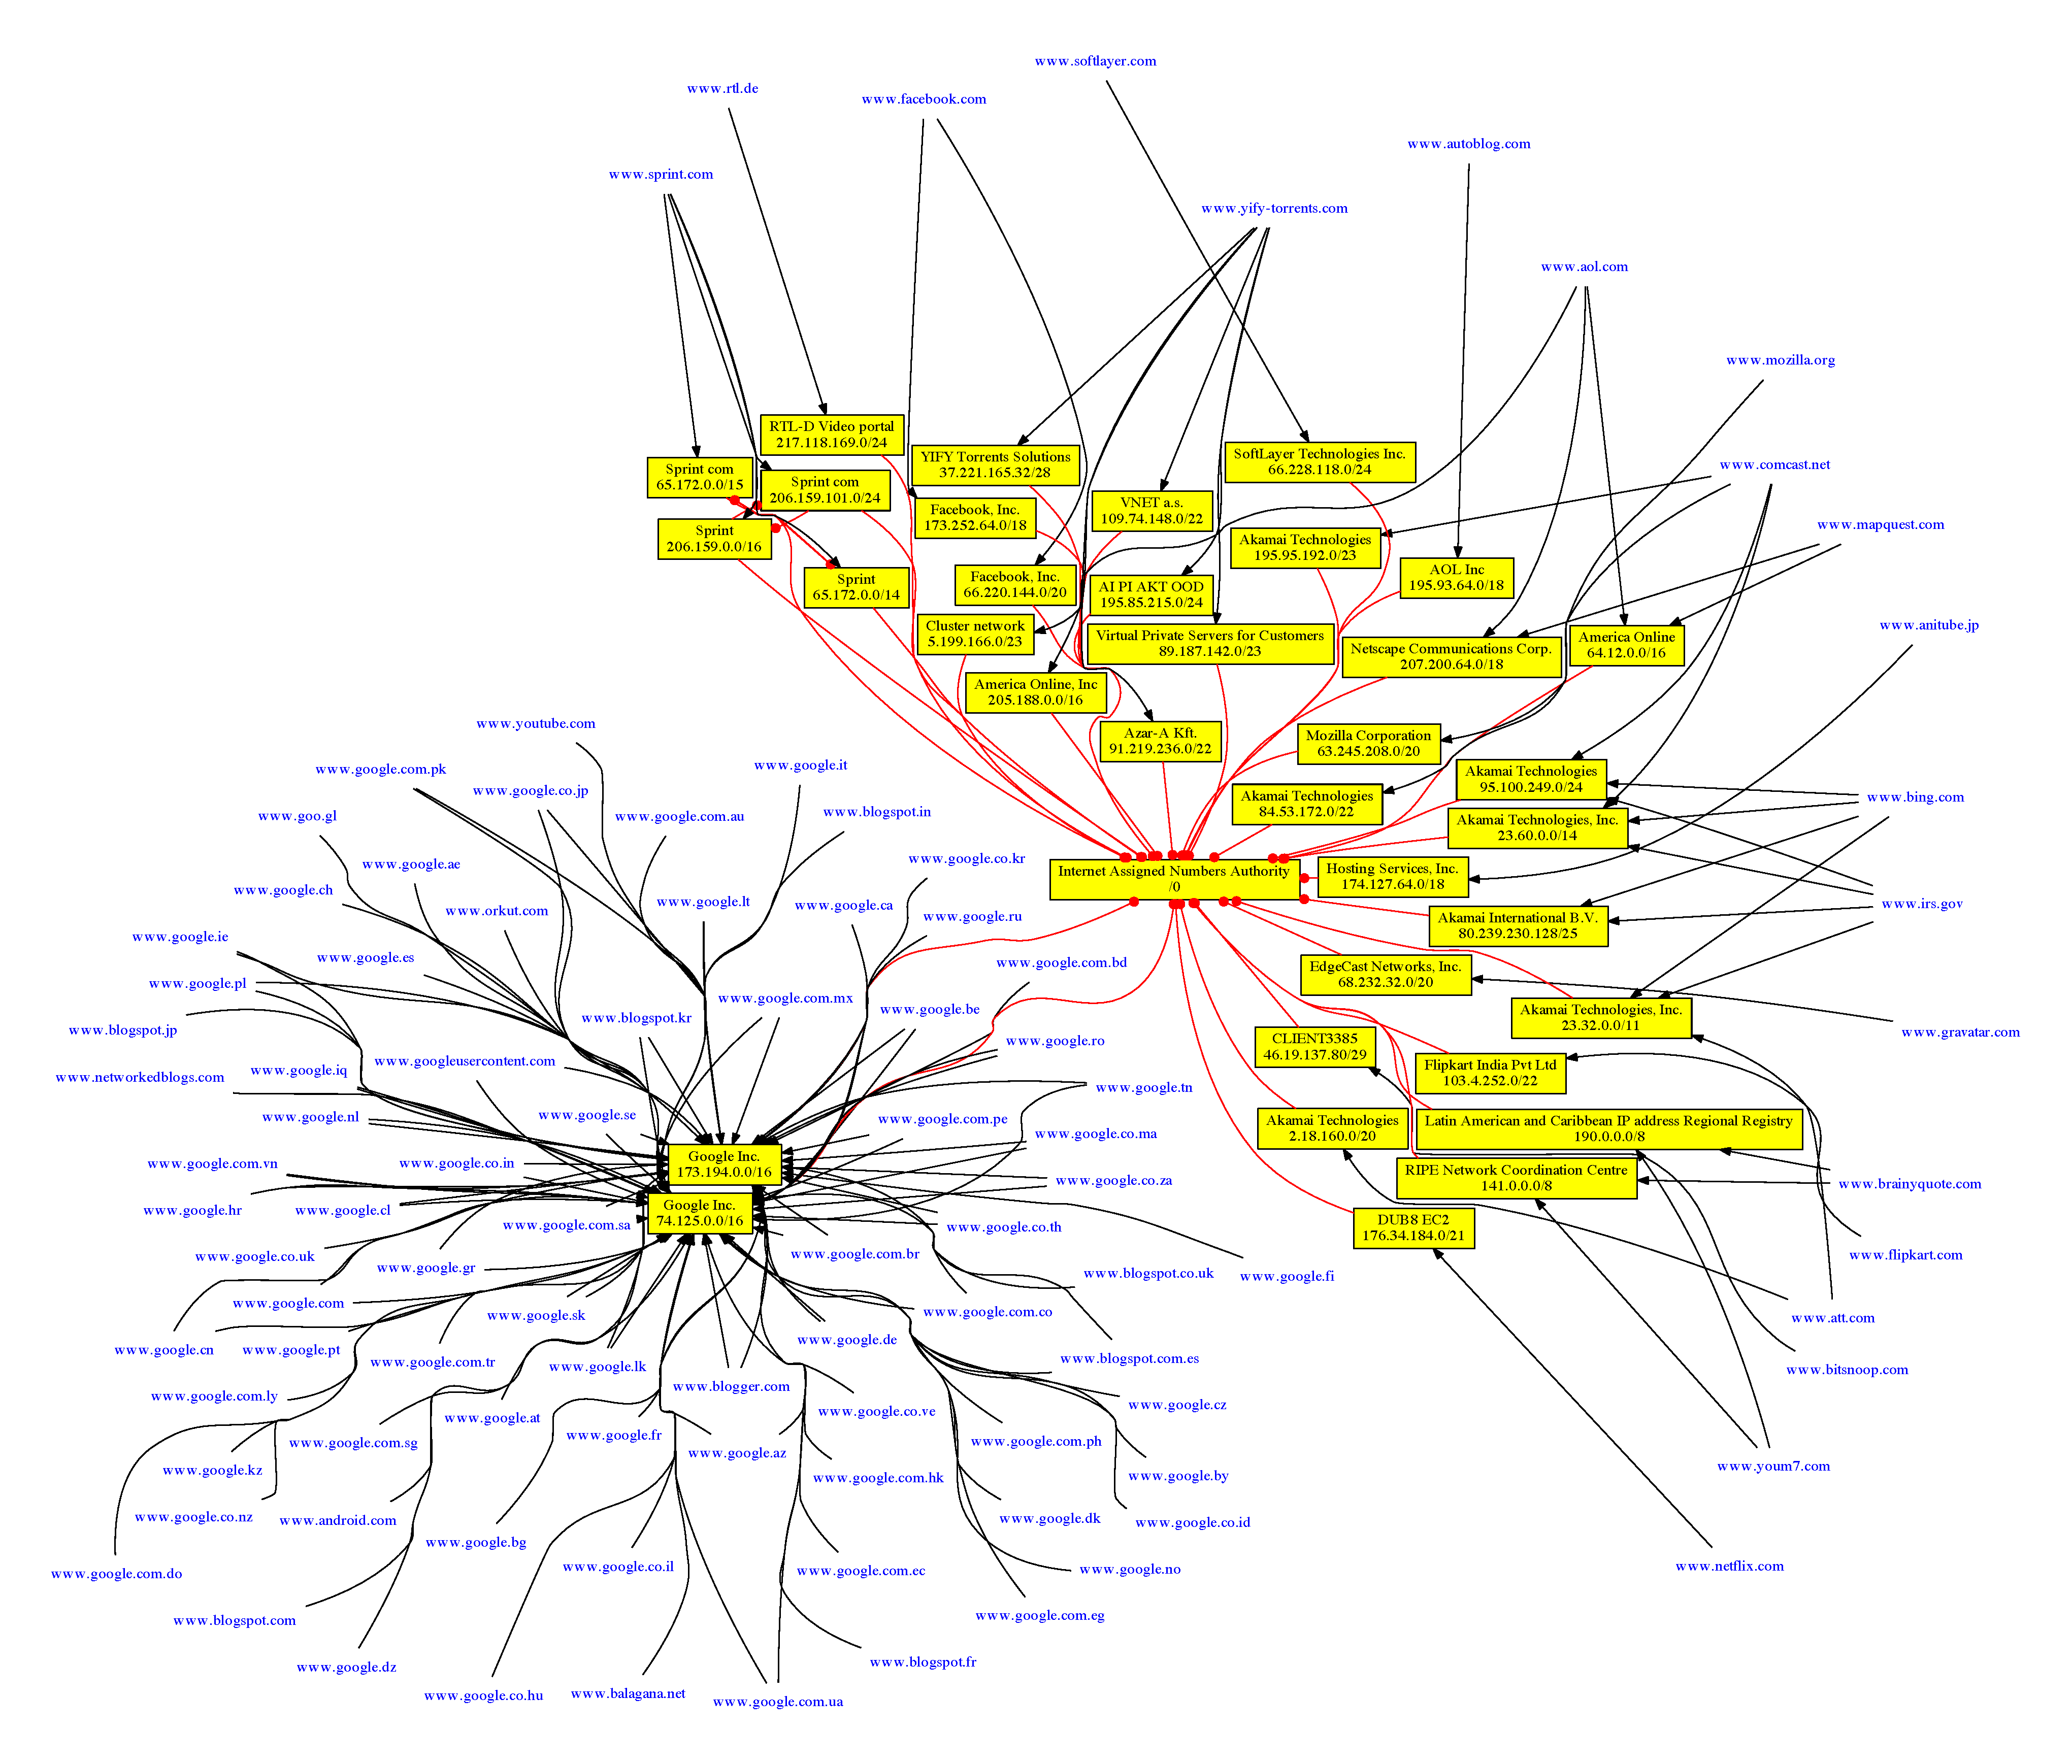
\includegraphics{figures/happy-v4cloud}}
  \end{minipage}
  \begin{minipage}[t]{0.50\textwidth}
    \centering
    \resizebox*{1.0\textwidth}{!}{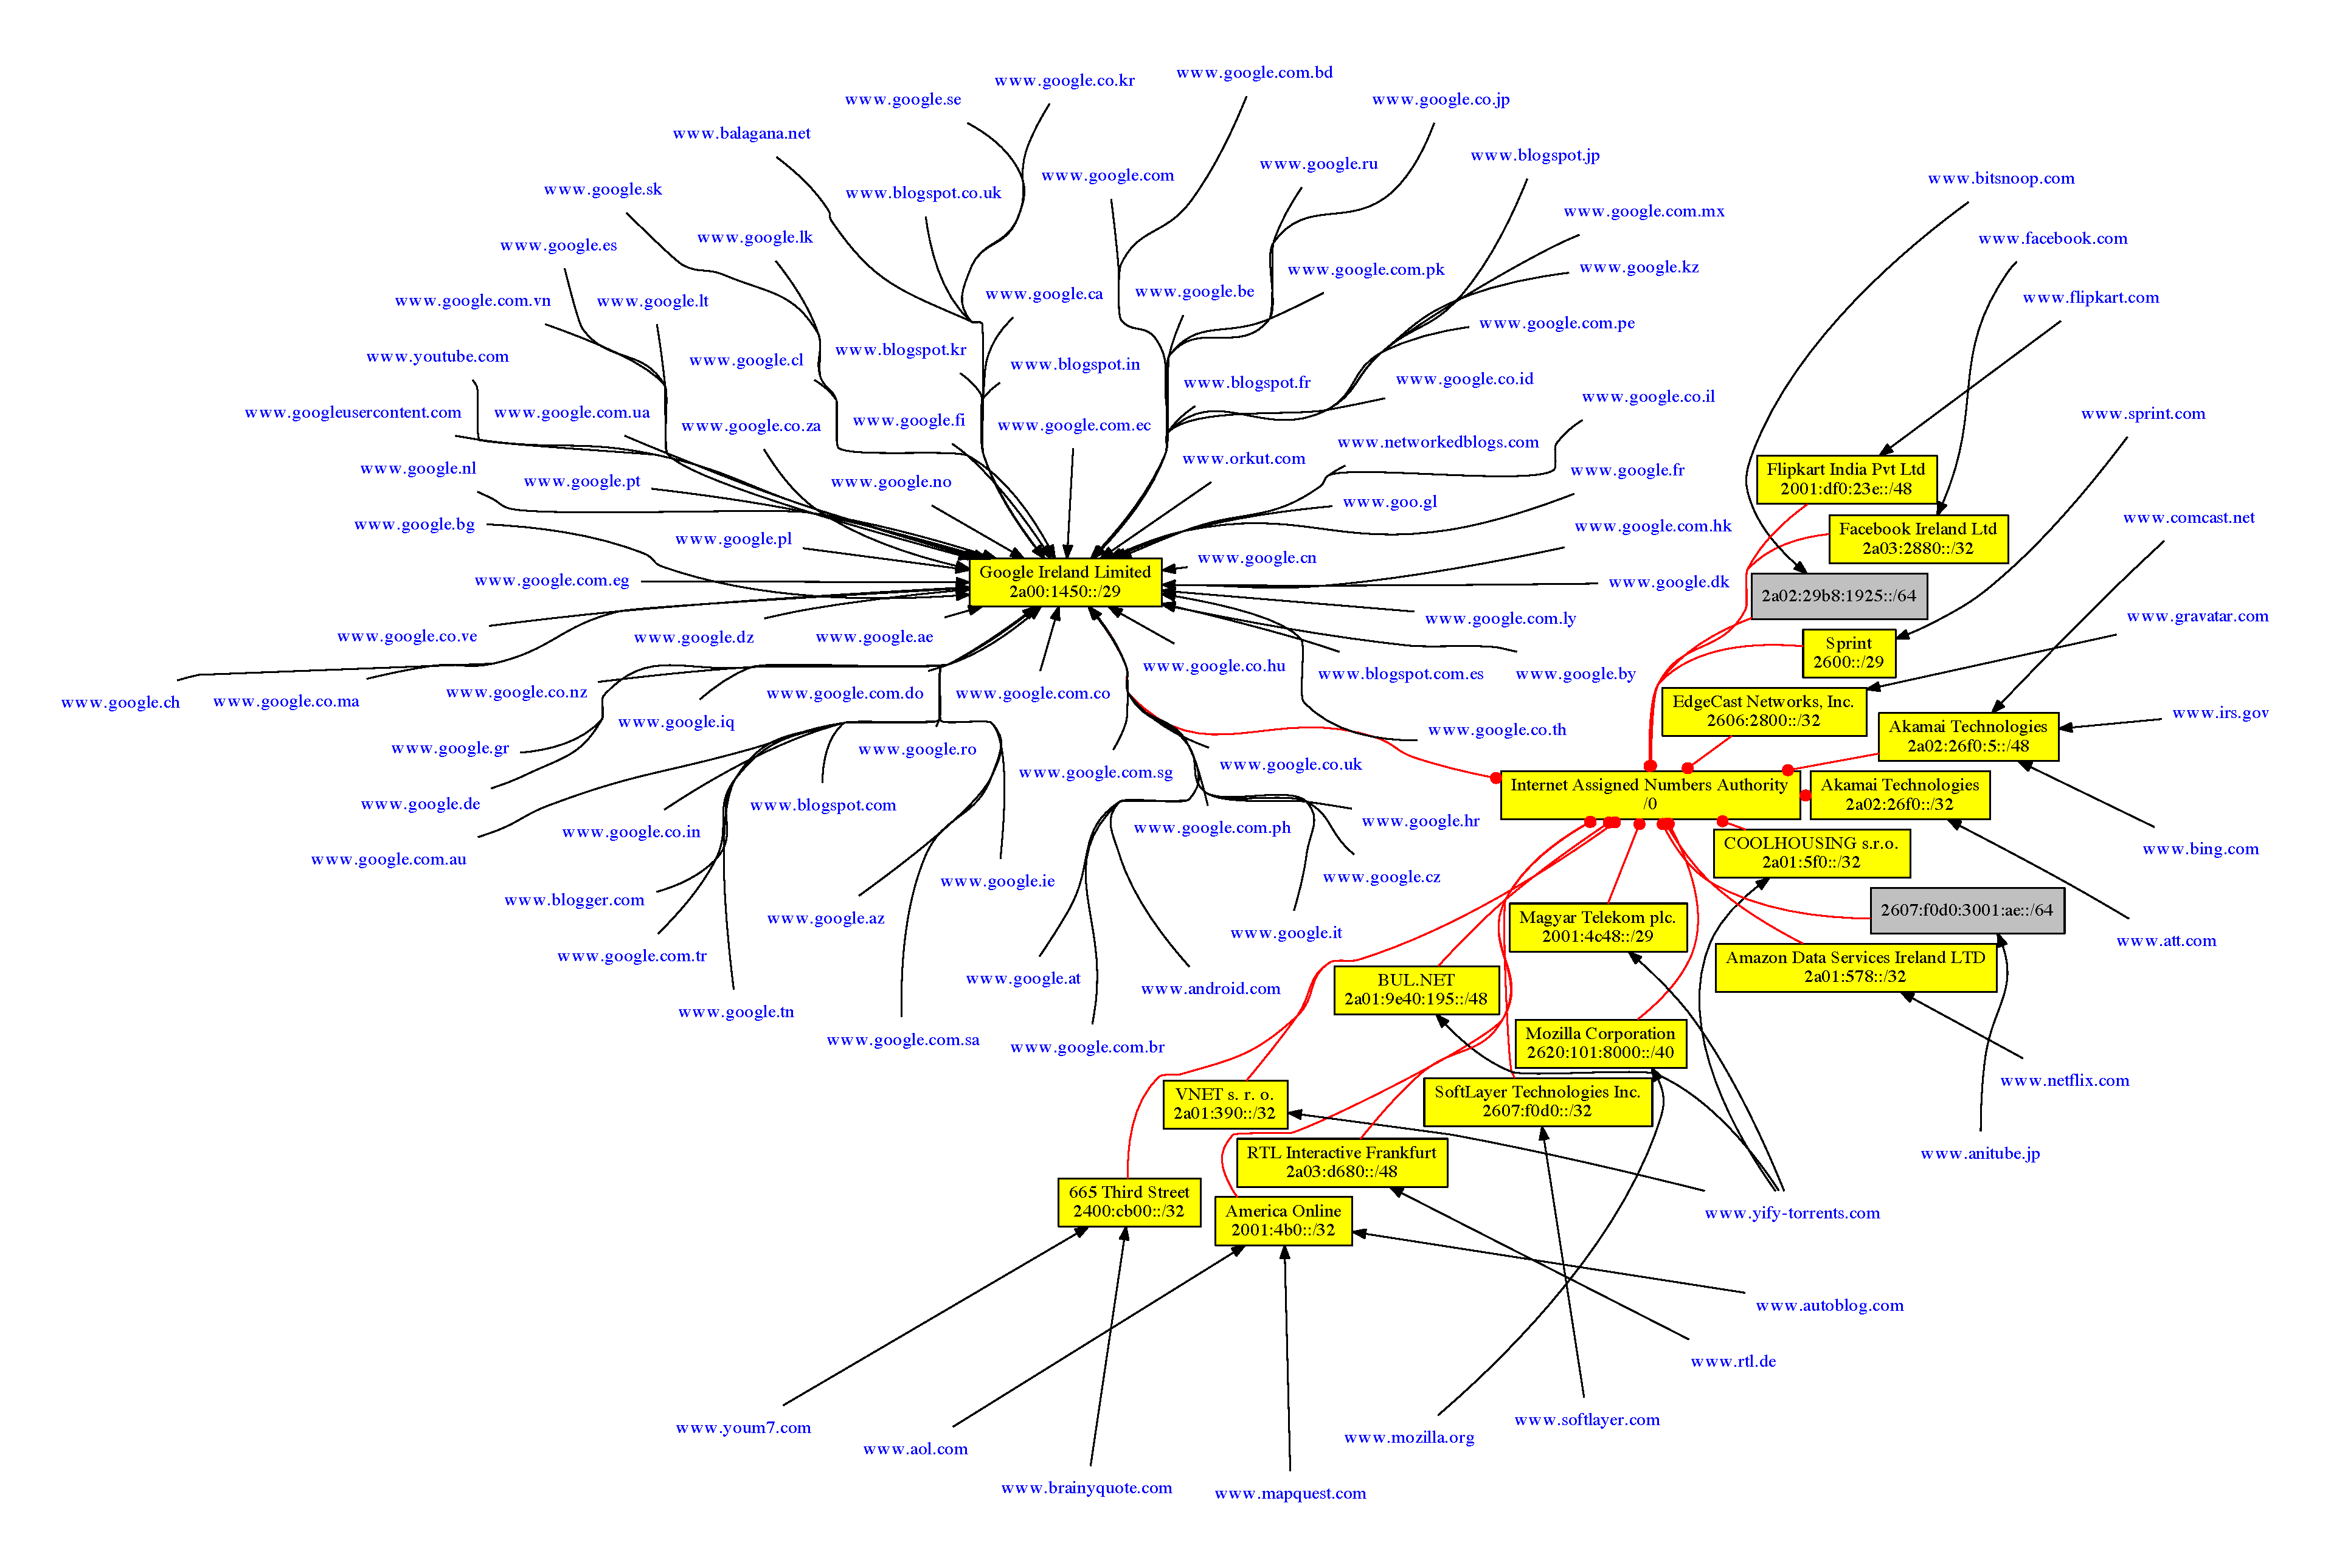
\includegraphics{figures/happy-v6cloud}}
  \end{minipage}
  \caption{\label{fig:v4-v6-cloud}An IPv4 (left) and IPv6 (right) aggregation
  cloud depicting how most of the services centralize on core \ac{CDN}s and
  major cloud platforms (zoom in to see the details).}
\end{figure}

A preliminary result comparing the mean time to establish a TCP connection to
each of the services from one of the measurement points is shown in Fig.
\ref{fig:t28972-mean}. The initial results show higher connection times over
IPv6. Furthermore, on a Teredo IPv6 measurement point, an application will
never use IPv6 except when IPv4 connectivity is broken, because the Teredo
IPv6 prefix has a low priority in the address selection algorithm
\cite{rfc6724}. In addition, it appears, several services show very similar
performance. These services either resolve to the same endpoint or a set of
endpoints that belong to the same allocated address blocks. Digging through
the \texttt{whois} information for each of the endpoints from their \ac{RIR}
seems to indicate that major portions of the services map to address blocks
owned by organizations such as Google and Akamai Technologies as shown in Fig.
\ref{fig:v4-v6-cloud}.
